\chapter{Conclusion \& Outlook}\label{ch:conclusion-outlook}
% Einleitung
This chapter discusses the insights acquired by exploring different techniques with the goal of the exploration of large unstructured text data.
% content
Firstly, in \autoref{subsec:discussion}, the results and findings are revised with respect to the research questions from \autoref{sec:research-questions}.
Then, \autoref{subsec:contribution} points out the scientific contributions. 
It is followed by \autoref{sec:outlook} which concludes with an outlook on the shortcomings of this thesis and future work.

\section{Conclusion}\label{sec:conclusion}

The insights of this work obtained from the examination of a variety of techniques are discussed in \autoref{subsec:discussion}.
Afterwards, the contributions of this work are summarized in \autoref{subsec:contribution}.


\subsection{Discussion}\label{subsec:discussion}

% preprocessing -> filter information
Before working with a model, the data has to be processed to a format that the model can work with.
The requirements imposed on the data format depend on the model.
Some models do not require any preprocessing, while others require a lot of preprocessing.

% tfidf preprocessing
Opposed to the other semantic embedding methods \ac{tfidf} requires preprocessing.
In this work, the \ac{tfidf} configuration includes the definition of a custom preprocessor.
Consequently, preprocessing plays an important role in this embedding.
The preprocessor is constructed with respect to the well-established preprocessing steps for \ac{nlp} tasks \cite{nlp-book2009},
the \ac{tfidf} documentation about the default preprocessor and the task.
Since the data set can contain figures due to the financial background, the preprocessor encodes all numbers into discrete strings.
Hence, the information is not lost but strongly reduced, which is vital due to the constraints imposed 
by the database's dense vector dimension limitation.
The custom preprocessor is compared to the default preprocessor on multiple datasets.
Since it consistently produces smaller vocabulary sizes, it is chosen for the task.

% visual preprocessing
The visual embedding methods also require preprocessing.
Originally, the images were matrices of \texttt{RGB} values.
However, \ac{pca} and \ac{optics} require a vector as input.
Therefore, the images are converted to greyscale and flattened to a vector.
The images are resized to make them more comparable.
Since clustering algorithms such as \ac{optics} encounter difficulties on high-dimensional data, 
applying \ac{pca} to compress the data can be considered preprocessing.


% compression: AE, PCA/ Eigendocs
As mentioned before, the database has a dense vector dimension limitation of 2048.
This limitation is a problem for the visual embedding methods as well as for \infersent{} and 
\ac{tfidf}.
The visual embedding methods are compressed with \ac{pca}, 
whereas the encoder of a trained \ac{ae} is employed for textual embeddings.
The \ac{pca} is fitted on 1000 randomly selected images.
The number of components is selected beforehand in consideration of the explained variance and the reconstruction error.
The architecture of the \ac{ae} is chosen in consideration of the reconstruction error on 195 documents.
However, both the \ac{pca} and the \ac{ae} model's quality would improve if they were trained on a larger dataset.


% visual vs semantic
As already stated this work examined both ways to encode semantic and visual information.
The evaluation is conducted with respect to the task of finding similar documents.
Since the data set is not labeled the evaluation is subjective and experimental.
Qualitative evaluation is conducted by inspecting the responses of different models for several sample queries to the database 
storing the respective embeddings.
The inspection is conducted manually, 
using Venn diagrams, heatmaps and 
statistical properties of the distribution of the cardinality of the shared query response sets.

The semantic responses are similar and often managed to find either documents with the same content or documents with the same company name.
The visual responses are more dissimilar from each other and the query document.
% visual: OPTICS, argmax
More precisely, the \texttt{argmax} approach returns poor results to some extent.
Consequently, \ac{optics} is considered the superior visual embedding method for the database.
Moreover, the textual embedding methods produce more meaningful responses than the visual embedding methods.
For example, textual embedding methods manage to find documents with the same company name, 
while visual embedding methods naturally return visually similar documents which not necessarily originated by the same company.


% semantic: TFIDF, Doc2Vec, USE, InferSent, SBERT
When evaluating the semantic embedding methods, slight differences between the models become evident.
Differences and similarities between the models are examined by comparing the responses to the sample queries.
This evaluation includes the calculation of the average portion of shared documents between the responses of several models 
and the exemplary evaluation of actual queries.
\ac{tfidf}, \ac{d2v} and \ac{sbert} are most dissimilar from each other.
The \ac{tfidf} approach performs rather poorly on unusual query documents such as handwritten documents.


% similarity: cosine
The similarity metric used in this work is cosine similarity.
Since \databaseName{} provides the similarity metrics Euclidean distance, dot product and cosine similarity,
one of these metrics had to be chosen.
Usually, cosine similarity is recommended for \ac{nlp} tasks and thus, applied in this work.
Soft cosine similarity is not used, since it is not available in \databaseName{}.
However, the usage of soft cosine would likely improve the results.

% topic analysis: wordclouds
Since the techniques discussed in this section have to be merged into a single system 
\wordcloud{} provides means to visualize the response documents containing the most similar documents for different models.
This approach is well suited to describe topics as groups of predominant words \cite{topic_modeling2019}.
The baseline topic analysis technique \ac{t2v} provides a \wordcloud{} implementation too.

% database: Elasticsearch
The database used in this work is \databaseName{}.
It was built to provide a fast and scalable search engine.
Moreover, it is a document-oriented database, which is well-suited for flexible data.
By default, several similarity measures and search strategies are provided.
Moreover, the elastic stack offers a wide range of tools supporting embedding models which are not used in this work.


% FE (Angular), BE (Flask)
The libraries used for the implementation of the tool are \angular{} and \flask{}.
The libraries were chosen after discussing options with this thesis' supervisor.
However, the implementation of this tool is not the focus of this work.

% top2vec
The baseline topic analysis technique \ac{t2v} is chosen due to its simplicity and functionalities.
The \ac{t2v} implementation is well documented and provides a \wordcloud{} implementation.
Moreover, it enables the user to find similar topics for query terms and returns inherent topics in a data corpus.
Hence, its functionality is similar to the functionality of the system developed in this work.

\subsection{Contribution}\label{subsec:contribution}
% mein Beitrag
% literature review, semantic -> visual
An exhaustive literature review was conducted to find suitable embedding methods for the task of finding similar documents.
Initially, only semantic embedding methods were considered.
However, when the first results were inspected the idea arose to group the documents by visual similarity.
Thus, visual embedding methods were included in the evaluation.

% using existing models
The semantic embedding methods were implemented using existing models.
All models offer adequate documentation and were thus, mostly comfortable to use.
However, some alterations had to be made to the models to make them suitable for the task.
For instance, a custom preprocessor was implemented for the \ac{tfidf} embedding method.
The preprocessor was a better fit for the task than the default preprocessor.
Moreover, a custom \ac{w2v} model was trained on the data set to be used by \infersent{}.
This reduced the time necessary to encode texts.

% eigenfaces -> eigendocs
The \eigenfaces{} approach has been prevalent since \citeyear{eigenfaces1991}.
In this work, the approach was adapted to the task of finding similar documents and thus, called \eigendocs{}.
The idea of projection items into a lower dimensional space was kept as well as the preprocessing steps.
However, the preprocessing was extended by placing the document images onto a white canvas.


% clustering
In order to find a suitable clustering algorithm for the task, literature research was conducted.
The research revealed that the \ac{optics} algorithm is a suitable candidate for the task.
In this work, two different preprocessing steps were implemented.
The first was similar to the preprocessing steps used in \cite{OPTICS1999}.
The second one utilized \eigendocs{} to reduce the dimensionality of the data set.
The parameters of the algorithm were chose in consideration of the reachability plot.


% pca components/ AE architecture evaluation
The data was compressed using \ac{pca} or the encoder of an \ac{ae}.
Both the \ac{pca} and \ac{ae} configurations were experimentally evaluated.
The number of components of the \ac{pca} was chosen in consideration of the cumulative explained variance 
and the reconstruction error.
The architecture of the \ac{ae} was chosen in consideration of the reconstruction error \ac{rsme} and 
the cosine similarity between the original and the reconstructed vector.


% database local & server
Before the data could be used for the task, it had to be stored in a database.
Firstly, the type of database had to be chosen.
It became clear that a document database would be the best fit for the task 
since it accepts documents of variable shape.
\databaseName{} is a well-known document database that is used by 
well-established companies successfully handling big data.
Secondly, the database had to be configured.
This required the consideration of different field types and similarity measures.
The dense vector seemed to be a native choice and cosine similarity was chosen 
among other reasons due to its popularity as a similarity metric in \ac{vsm}.
Afterwards scripts to store the data in the database were implemented.
The local database stores 2048 randomly chosen documents from the whole data set.
The server database currently stores around $497504$ incomplete documents.

% evaluation: venn & heatmap, mean/ std
Since the dataset is not labeled, the evaluation of the results is not trivial.
Therefore, multiple evaluation methods were implemented.
The first method is a Venn diagram that shows the intersection of the results of the power set of different methods.
The second method is a heatmap that shows the average portion of shared response documents between different methods.
Lastly, the mean and standard deviation of the portion of shared response documents were calculated 
to further investigate the distribution of the results obtained above.

% topic modeling
To ensure \wordcloud{}s display only valid words the tokens were lemmatized before applying the \wordcloud{}. 
The existing functionalities implemented by the library \topTwovec{} were bundled into a class 
which accepts inputs native to the task at hand.
Hence, the functionalities were not extended but rather adapted to the task.  


% chapter about motivation -> goals, techniques used and COMBINED
As initially mentioned, this thesis aims to provide computational means to facilitate the work with large unstructured text data.
In the course of this work, multiple \ac{ml} techniques were examined and evaluated on the task of finding similar documents.
The semantic embedding methods \ac{tfidf}, \ac{d2v}, \infersent{}, \ac{use} and \ac{sbert} were examined.
\eigendocs{} was implemented as a visual embedding method.
It was possible to find a suitable database to store the data.
A pipeline to preprocess, embed and store the data in the database was developed.
The pipeline is scalable to large datasets.
However, models such as \ac{tfidf} yield less meaningful results on certain query documents and 
are prone to performance deterioation with increasing document corpus, since the embeddings' 
dimensionality correlates directly with the vocabulary size.
When the number of terms in the data corpus increases, but the vocabulary size is static, 
it is likely that the vocabulary lacks important words. 

Moreover, a tool was implemented.
The tool provides the possibility to conduct text queries.
A document of interest can be examined in more detail:
The detail component not only contains a \ac{pdf} viewer, 
a \wordcloud{} of the most frequent words in the document, but also an option to examine the query responses for different embeddings.
The file names of the ten most similar documents and a \wordcloud{} of the most frequent words among those documents is displayed.

An experimental evaluation of the embeddings was conducted.
The visual embedding methods were found to be inferior to the semantic embedding methods on certain query documents.
The tool was compared to a baseline topic modeling approach called \topTwovec{}.
The library \topTwovec{} implemented similar functionalities.
However, the tool is not designed for a productive environment since the focus is on the comparison of different models rather than usability.


\section{Outlook}\label{sec:outlook}
% features of the application

% What did I find?
When investigating both semantic and visual embedding methods, differences between the models became evident.
Overall, the textual embedding methods produced more meaningful responses than the visual embedding methods.
However, this is not surprising since the textual embedding methods prioritize documents containing equal or semantically similar terms and thus,
return documents of similar content or originating from the same company as the query document.
Visual embedding methods, on the other hand, return visually similar documents.

It is complicated to compare the responses of semantic and visual embedding methods since they operate on fundamentally different data.
A more thorough evaluation could include a survey.
A selection of the results of this work is incorporated into the first approach to constructing a survey.
13 people with different academic backgrounds have partaken in the survey.
A question and result from the survey are displayed in \autoref{fig:survey}.
However, constructing a survey is complicated since semantic similarities should be evaluated on a textual level, i. e. content, 
which is difficult for non-experts and not natural since humans are prone to assess similarities by visual inspection.
Moreover, identification of the target audience is difficult since the target audience of the tool could be expanded to be more general than the tax office.

\begin{figure}%
    \centering
    \subfloat[\centering A question of the survey.]{{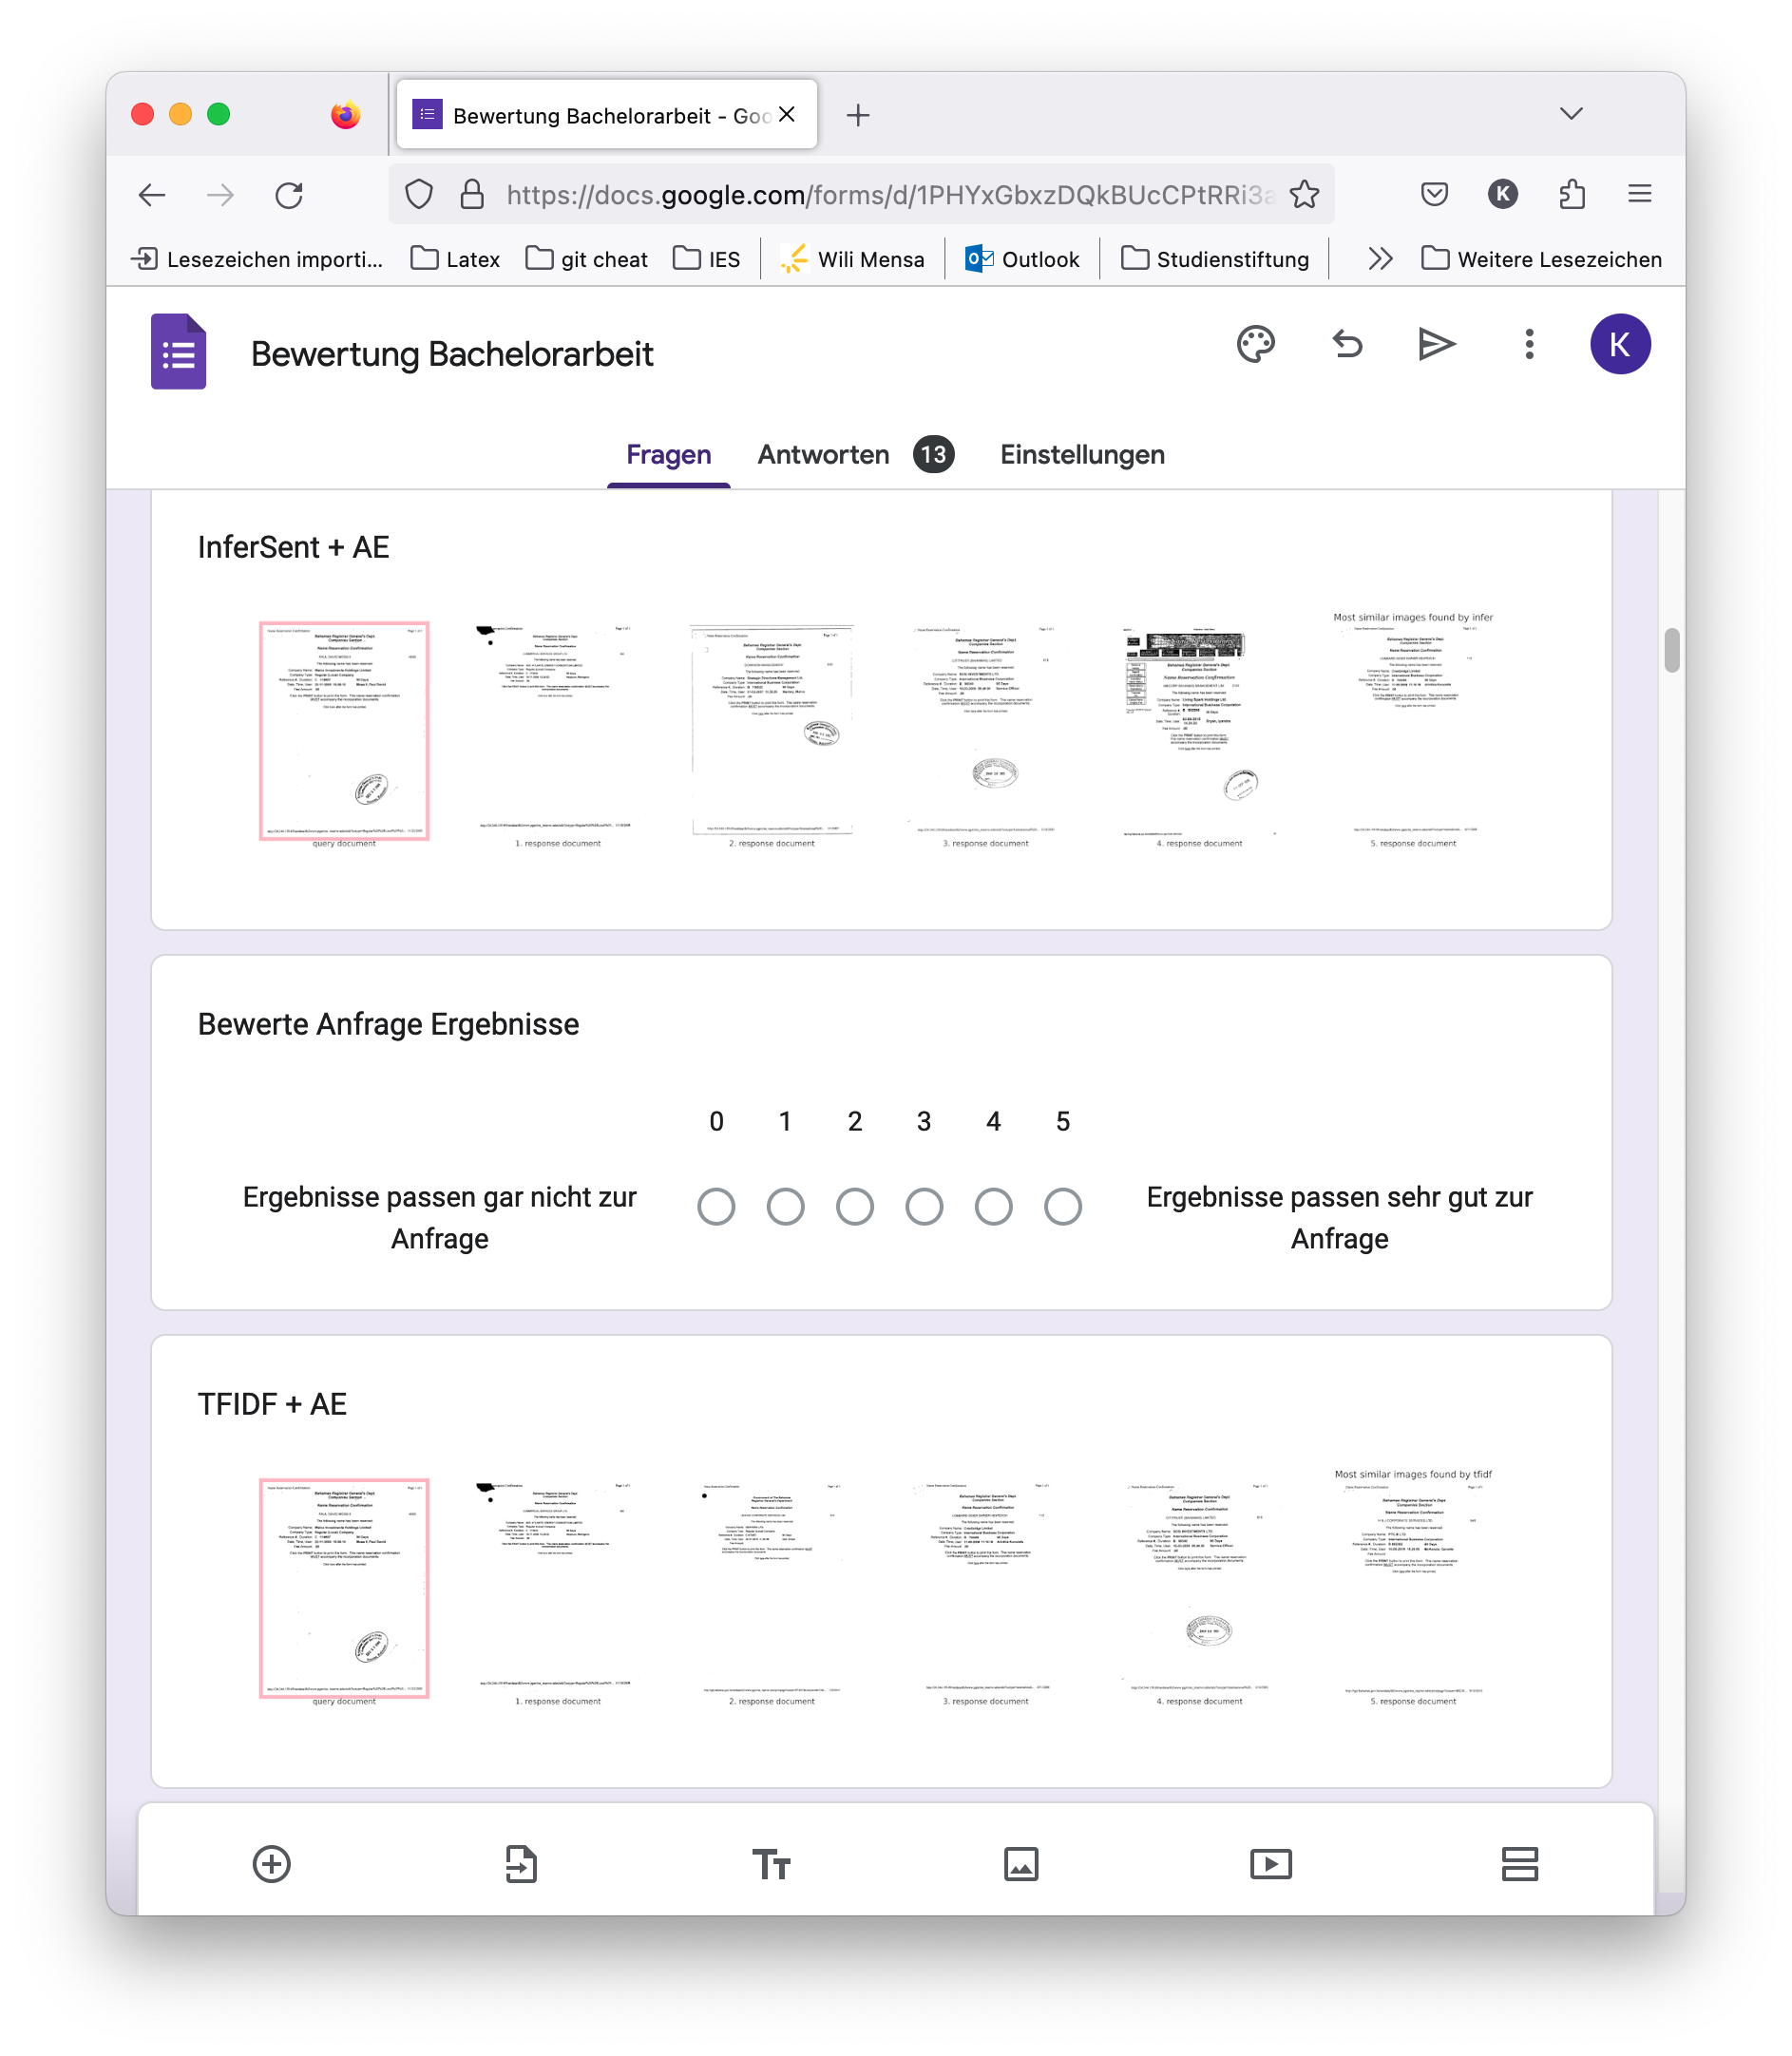
\includegraphics[width=5cm]{images/Umfrage/Umfrage_ex.png} }}%
    \qquad
    \subfloat[\centering Selection of results of survey.]{{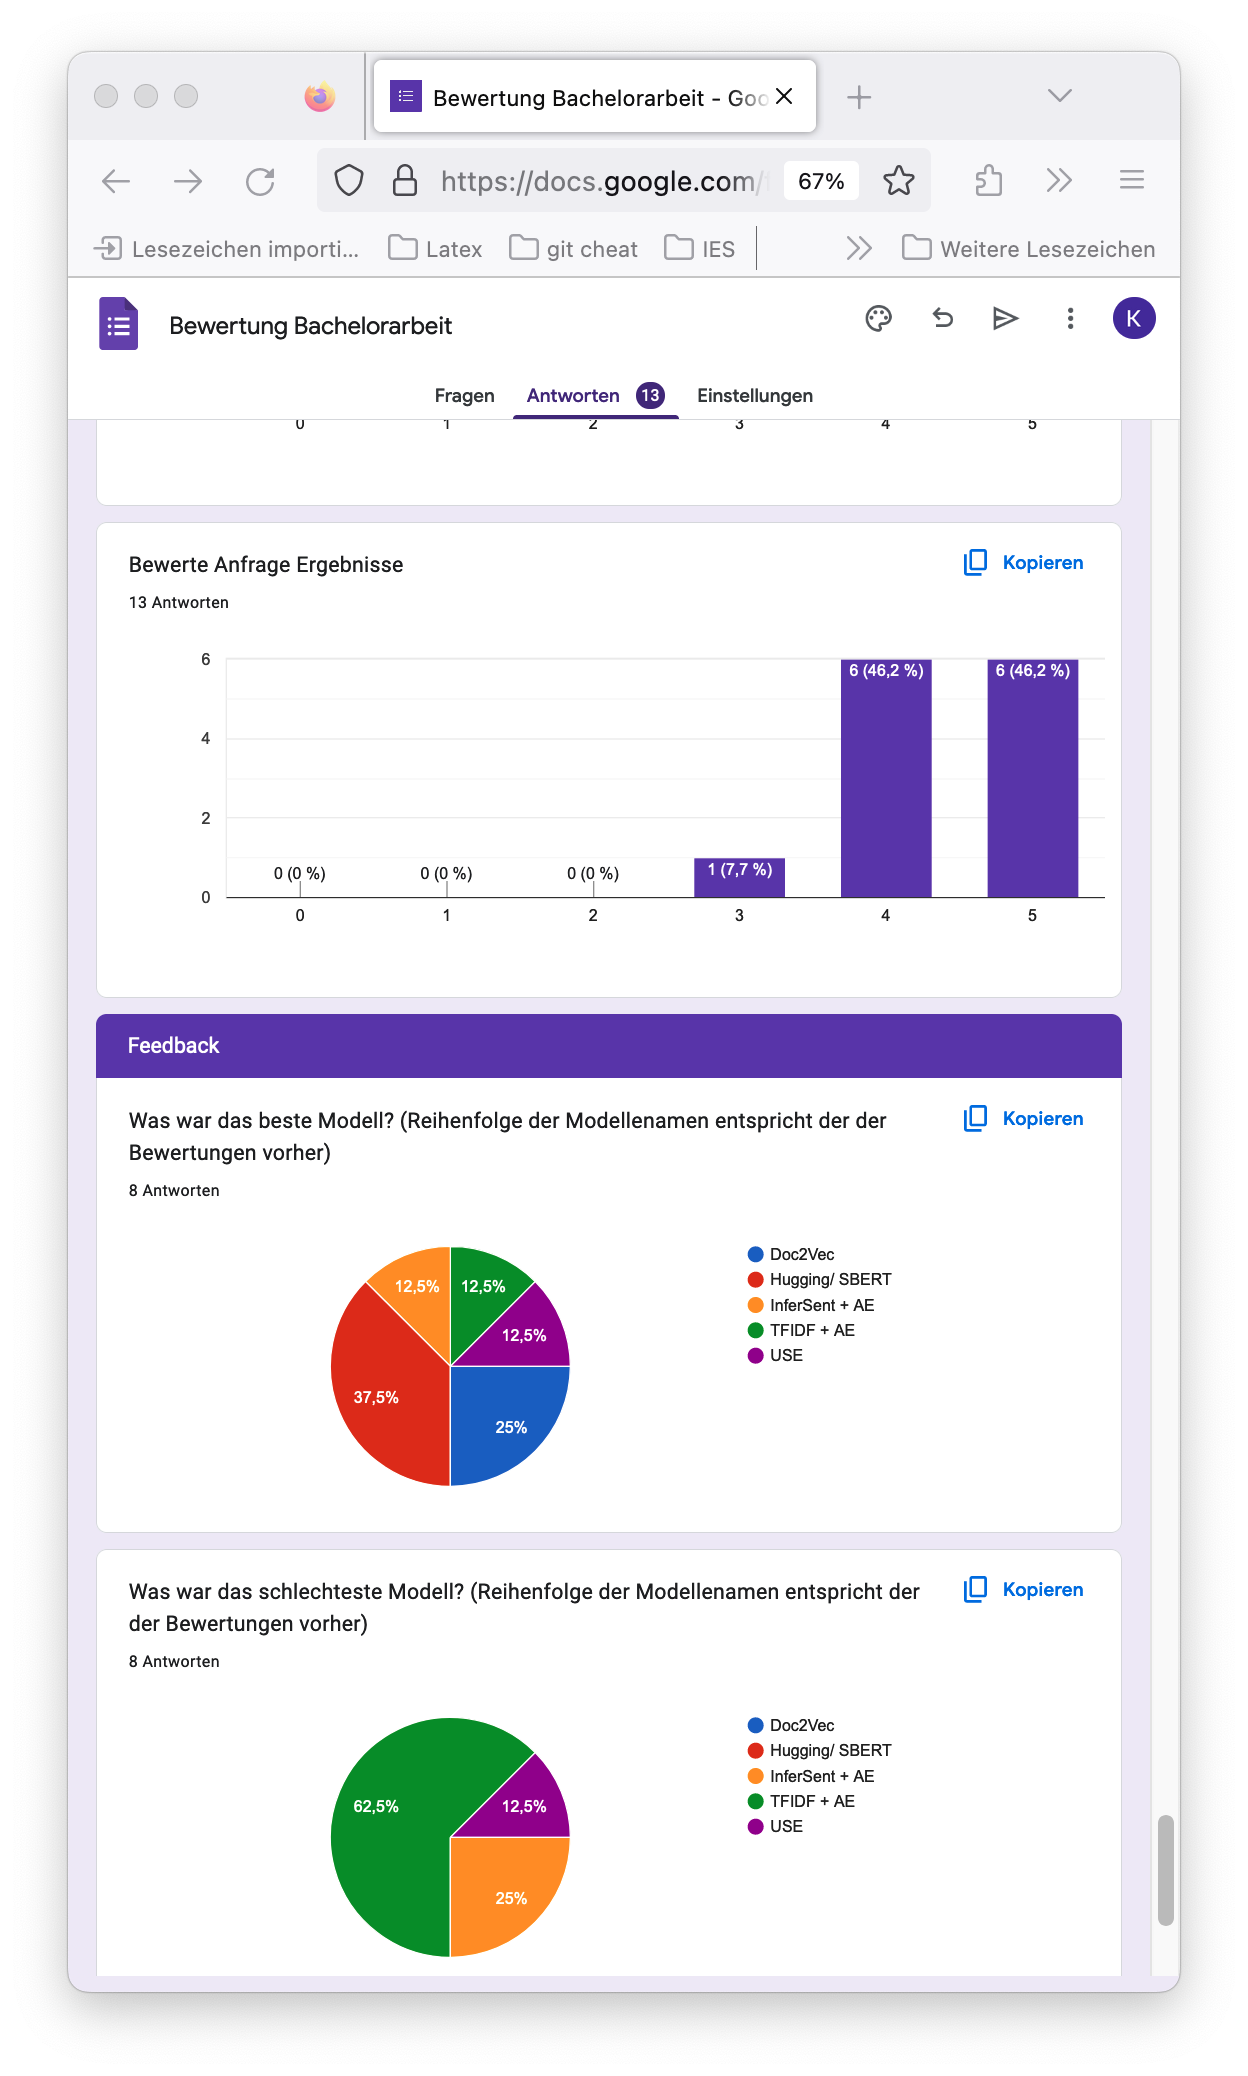
\includegraphics[width=5cm]{images/Umfrage/Umfrage_erg.png} }}%
    \caption[Survey approach]{A first survey approach from \cite{BA-survey}.}%
    \label{fig:survey}%
\end{figure}

% Problems/ critic
% Embedding methods
% hyperparameter tuning
Similar to \citeauthor{glove2014}'s work, in this thesis, for many models used, any unspecified parameters are set to their default values, 
assuming that they are close to optimal
acknowledging that this simplification should be revised in a more thorough analysis.

% TFIDF
The \ac{tfidf} approach performs rather poorly on unusual query documents.
There are multiple factors that could have contributed to this result.
Firstly, the vocabulary is drastically reduced to satisfy the database's constraints for dense vector dimensionality.
Thus, \ac{tfidf} may either be unsuitable for the task of finding similar documents when the vocabulary size is restricted or 
further research is required to find more suitable means to compress the embedding before inserting it into the database.
Secondly, the evaluation of the different preprocessors of \ac{tfidf} is carried out on small datasets of 195 and 2048 documents.
This dataset may not be representative of the whole corpus.

% GloVe (InferSent)
In this work, the precomputed \ac{glove} embeddings are replaced by a custom \ac{w2v} model.
However, \citeauthor{glove2014} state that \acs{glove} outperforms \ac{w2v} on the same corpus, 
vocabulary and window size in terms of quality \cite{glove2014}.
Hence, the quality of \infersent{} might have deteriorated due to the replacement of \ac{glove} by \ac{w2v}.

% Visual embedding methods
% Eigendocs
When preprocessing the document images for \eigendocs{}, the images are placed on a white canvas assuming 
its dimensions are bigger or equal to all other documents in the corpus.
Since this assumption was not true, the images selected to find the dimensionalities of the canvas are not representative.

% compression: PCA
The parameter selection for \ac{pca} is not representative of the whole dataset, 
due to the fact that the dataset used for the evaluation error was not drawn randomly from the data corpus and is too small.
Moreover, the resulting plot is not optimal for conducting the "elbow method", since no significant change is evident in the slope.


% AE config: Problem & future work
Different \ac{ae} architectures are experimentally evaluated on a selection of 195 documents.
However, since the dataset is too small and not drawn randomly from the whole data corpus the results are not representative.
Thus, future work should include a more thorough evaluation of different \ac{ae} architectures on a bigger document corpus.
% tfidf + AE only used on server

% comparison on training data
The comparison of the different embedding methods in terms of query response similarity was carried out on the data which was stored in the database.
For future work, the comparison should be carried out on a separate data set to evaluate the performance of the models on unseen data.

% eval weights of response documents
The evaluation of the similarity between query results of different models so far 
has not considered the individual weights for respective query responses
because it was difficult to find means 
to interpret and visualize semantic meaningful weight relationships.
Thus, future work could include the weights of the query responses in the evaluation.

% similarity of query documents
Moreover, the similarity of the query documents is not considered in the evaluation.
To further improve the evaluation, the number of occurrences of query documents in the response documents of other queries could be examined.

% elastic stack: Kibana
The elastic stack offers a wide range of tools, for instance, Kibana that can be used to manage models and 
to create ingest pipelines to embed new documents.
If models are managed by Kibana, the models no longer have to be managed by the user and thus, 
the system would most likely be more user-friendly and less prone to errors.

% server database
Another issue is the fact that the database contains neither all embeddings nor all documents.
The Bahamas leak contains 38 \ac{gb} of data.
Even though multiprocessing using Pool is used to split the workload across up to 100 processes, 
the embedding process is not finished after several days.
Hence, more advanced coding techniques have to be applied to speed up the embedding process.

% Future: continue developing this application with the tax office
The domain of financial fraud and tax evasion is very interesting.
Thus, future work could include the development of a working system for the tax office.
The techniques explored in this work could be used to find similar documents to a query document and thus,
facilitate initial exploration of a large data corpus.
However, the tool developed in this work is not yet ready to be used in tax offices.
The different embedding models to choose from are useful for research purposes but not in a productive environment.